% Atom, description, circuit, SKETCH
\appendix
\section{SKETCH code and circuit diagrams for atoms}
The appendix provides circuit diagrams (Figures~\ref{fig:rw}--~\ref{fig:pairs})
and SKETCH code (Table~\ref{tab:atom_code}) for the atoms in
Table~\ref{tab:templates}. Table~\ref{tab:sketch_constructs} summarizes the
SKETCH notation we use in this section.
\begin{table}[!htbp]
  \begin{scriptsize}
  \begin{tabular}{p{0.3\columnwidth}p{0.7\columnwidth}}
  SKETCH construct & Description \\
  \hline
  MuxN(a1, a2, \dots, aN) & \pbox{0.7\columnwidth}{N-to-1 multiplexer with enable bit.\\If enabled, return one of a1, a2, \dots aN.\\If disabled, return 0.}\\
  Opt(a)        & Return a or 0. \\
  rel\_op(x, y) & Return one of $x < y$, $x > y$, $x != y$, $x == y$.\\
  Const() & Return an integer constant in the range [0, 31].\footnote{We restrict constants to 5 bits because all constants in our dataplane algorithms are under 32. Larger ranges increase synthesis time.} \\
  x, y & State variables \\
  pkt\_1, pkt\_2 & Packet fields \\
  \end{tabular}
  \end{scriptsize}
  \caption{SKETCH notation used in atom templates}
  \label{tab:sketch_constructs}
\end{table}
\begin{table*}[!htbp]
\begin{scriptsize}
  \center
  \begin{tabular}{|p{0.09\textwidth}|p{0.73\textwidth}|p{0.04\textwidth}|}
      \hline
      Atom & Atom template & Element depth\\
\hline
\pbox{0.1\textwidth}{Write\\Figure~\ref{fig:rw}} &
{\begin{lstlisting}[style=customctable]
x = Mux2(pkt_1, Const());
\end{lstlisting}} &
1 \\

\hline
\pbox{0.1\textwidth}{ReadAddWrite\\(RAW)\\Figure~\ref{fig:raw}} &
{\begin{lstlisting}[style=customctable]
x = Opt(x) + Mux2(pkt_1, Const());
\end{lstlisting}} &
2 \\

\hline
\pbox{0.1\textwidth}
{Predicated\\
ReadAddWrite\\(PRAW)\\Figure~\ref{fig:praw}} &
{\begin{lstlisting}[style=customctable]
if (rel_op(Opt(x), Mux3(pkt_1, pkt_2, Const()))) {
  x = Opt(x) + Mux3(pkt_1, pkt_2, Const());
}
\end{lstlisting}} &
3 \\

\hline
\pbox{0.1\textwidth}
{If-Else\\
ReadAddWrite\\(IfElseRAW)\\Figure~\ref{fig:ifelseraw}} &
{\begin{lstlisting}[style=customctable]
if (rel_op(Opt(x), Mux3(pkt_1, pkt_2, Const()))) {
  x = Opt(x) + Mux3(pkt_1, pkt_2, Const());
} else {
  x = Opt(x) + Mux3(pkt_1, pkt_2, Const());
}
\end{lstlisting}} &
3 \\

\hline
\pbox{0.1\textwidth}
{Subtract (Sub)\\Figure~\ref{fig:sub}} &
{\begin{lstlisting}[style=customctable]
if (rel_op(Opt(x), Mux3(pkt_1, pkt_2, Const()))) {
  x = Opt(x) + Mux3(pkt_1, pkt_2, Const()) - Mux3(pkt_1, pkt_2, Const());
} else {
  x = Opt(x) + Mux3(pkt_1, pkt_2, Const()) - Mux3(pkt_1, pkt_2, Const());
}
\end{lstlisting}}&
4 \\

\hline
\pbox{0.1\textwidth}
{Nested Ifs\\(Nested)\\Figure~\ref{fig:nested}} &
{\begin{lstlisting}[style=customctable]
if (rel_op(Opt(x) + Mux2(pkt_1, pkt_2) - Mux2(pkt_1, pkt_2), Const())) {
 if (rel_op(Opt(x) + Mux2(pkt_1, pkt_2) - Mux2(pkt_1, pkt_2), Const())) {
  x = Opt(x) + Mux3(pkt_1, pkt_2, Const()) - Mux3(pkt_1, pkt_2, Const());
 } else {
  x = Opt(x) + Mux3(pkt_1, pkt_2, Const()) - Mux3(pkt_1, pkt_2, Const());
 }
} else {
 if (rel_op(Opt(x) + Mux2(pkt_1, pkt_2) - Mux2(pkt_1, pkt_2), Const())) {
  x = Opt(x) + Mux3(pkt_1, pkt_2, Const()) - Mux3(pkt_1, pkt_2, Const());
 } else {
  x = Opt(x) + Mux3(pkt_1, pkt_2, Const()) - Mux3(pkt_1, pkt_2, Const());
 }
}
\end{lstlisting}} &
6 \\

\hline
\pbox{0.1\textwidth}
{Paired Updates\\(Pairs)\\Figure~\ref{fig:pairs}} &
{\begin{lstlisting}[style=customctable]
if (rel_op(Mux2(x, y) + Mux2(pkt_1, pkt_2) - Mux2(pkt_1, pkt_2), Const())) {
 if (rel_op(Mux2(x, y) + Mux2(pkt_1, pkt_2) - Mux2(pkt_1, pkt_2), Const())) {
  x = Opt(x) + Mux3(pkt_1, pkt_2, Const()) - Mux3(pkt_1, pkt_2, Const());
  y = Opt(y) + Mux3(pkt_1, pkt_2, Const()) - Mux3(pkt_1, pkt_2, Const());
 } else {
  x = Opt(x) + Mux3(pkt_1, pkt_2, Const()) - Mux3(pkt_1, pkt_2, Const());
  y = Opt(y) + Mux3(pkt_1, pkt_2, Const()) - Mux3(pkt_1, pkt_2, Const());
 }
} else if (rel_op(Mux2(x, y) + Mux2(pkt_1, pkt_2) - Mux2(pkt_1, pkt_2), Const())) {
 if (rel_op(Mux2(x, y) + Mux2(pkt_1, pkt_2) - Mux2(pkt_1, pkt_2), Const())) {
  x = Opt(x) + Mux3(pkt_1, pkt_2, Const()) - Mux3(pkt_1, pkt_2, Const());
  y = Opt(y) + Mux3(pkt_1, pkt_2, Const()) - Mux3(pkt_1, pkt_2, Const());
 } else {
  x = Opt(x) + Mux3(pkt_1, pkt_2, Const()) - Mux3(pkt_1, pkt_2, Const());
  y = Opt(y) + Mux3(pkt_1, pkt_2, Const()) - Mux3(pkt_1, pkt_2, Const());
 }
}
\end{lstlisting}} &
6 \\
\hline

  \end{tabular}
  \end{scriptsize}
  \caption{SKETCH code for atoms described in Table~\ref{tab:templates}}
  \label{tab:atom_code}
\end{table*}


\newpage 
\begin{figure*}[!htbp]
  \center
  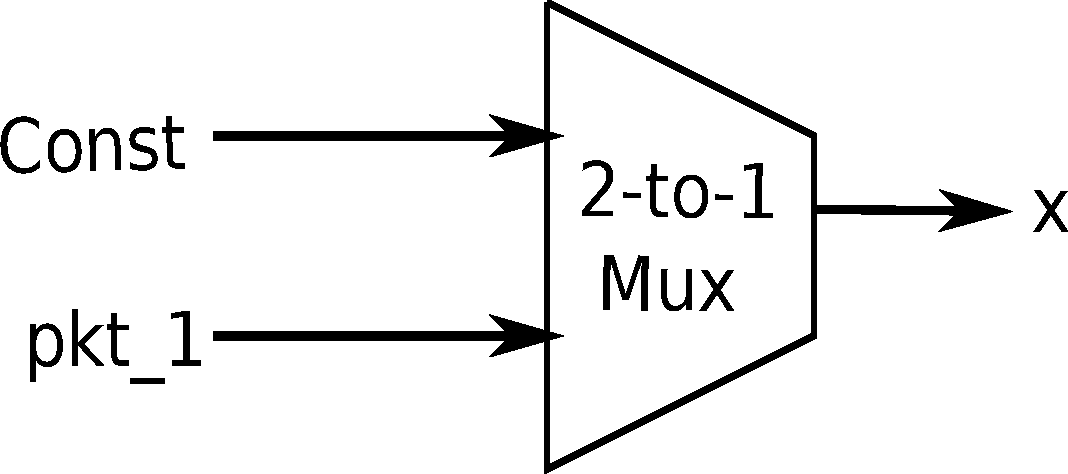
\includegraphics[width=\columnwidth]{rw.pdf}
  \caption{Circuit for Write atom with depth 1.}
  \label{fig:rw}
\end{figure*}
\begin{figure*}[!htbp]
  \center
  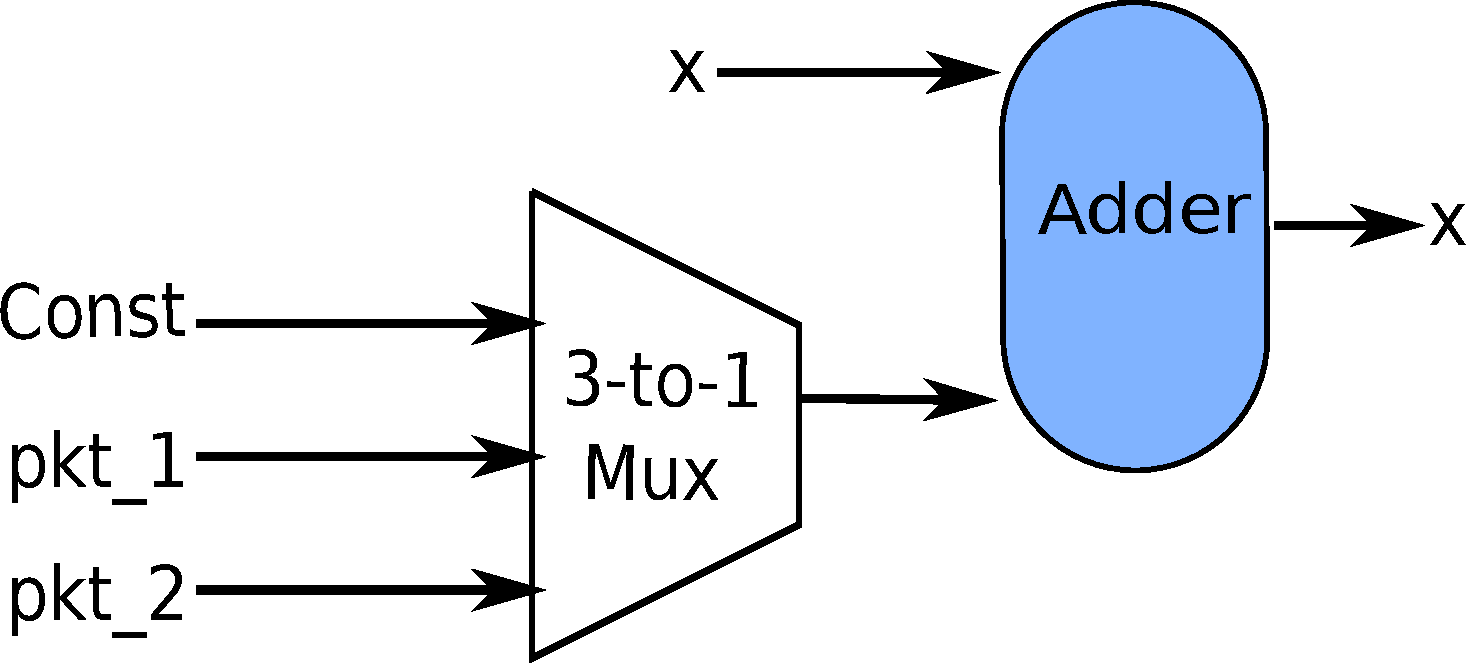
\includegraphics[width=\columnwidth]{raw.pdf}
  \caption{Circuit for RAW atom with depth 2.}
  \label{fig:raw}
\end{figure*}
\begin{figure*}[!htbp]
  \center
  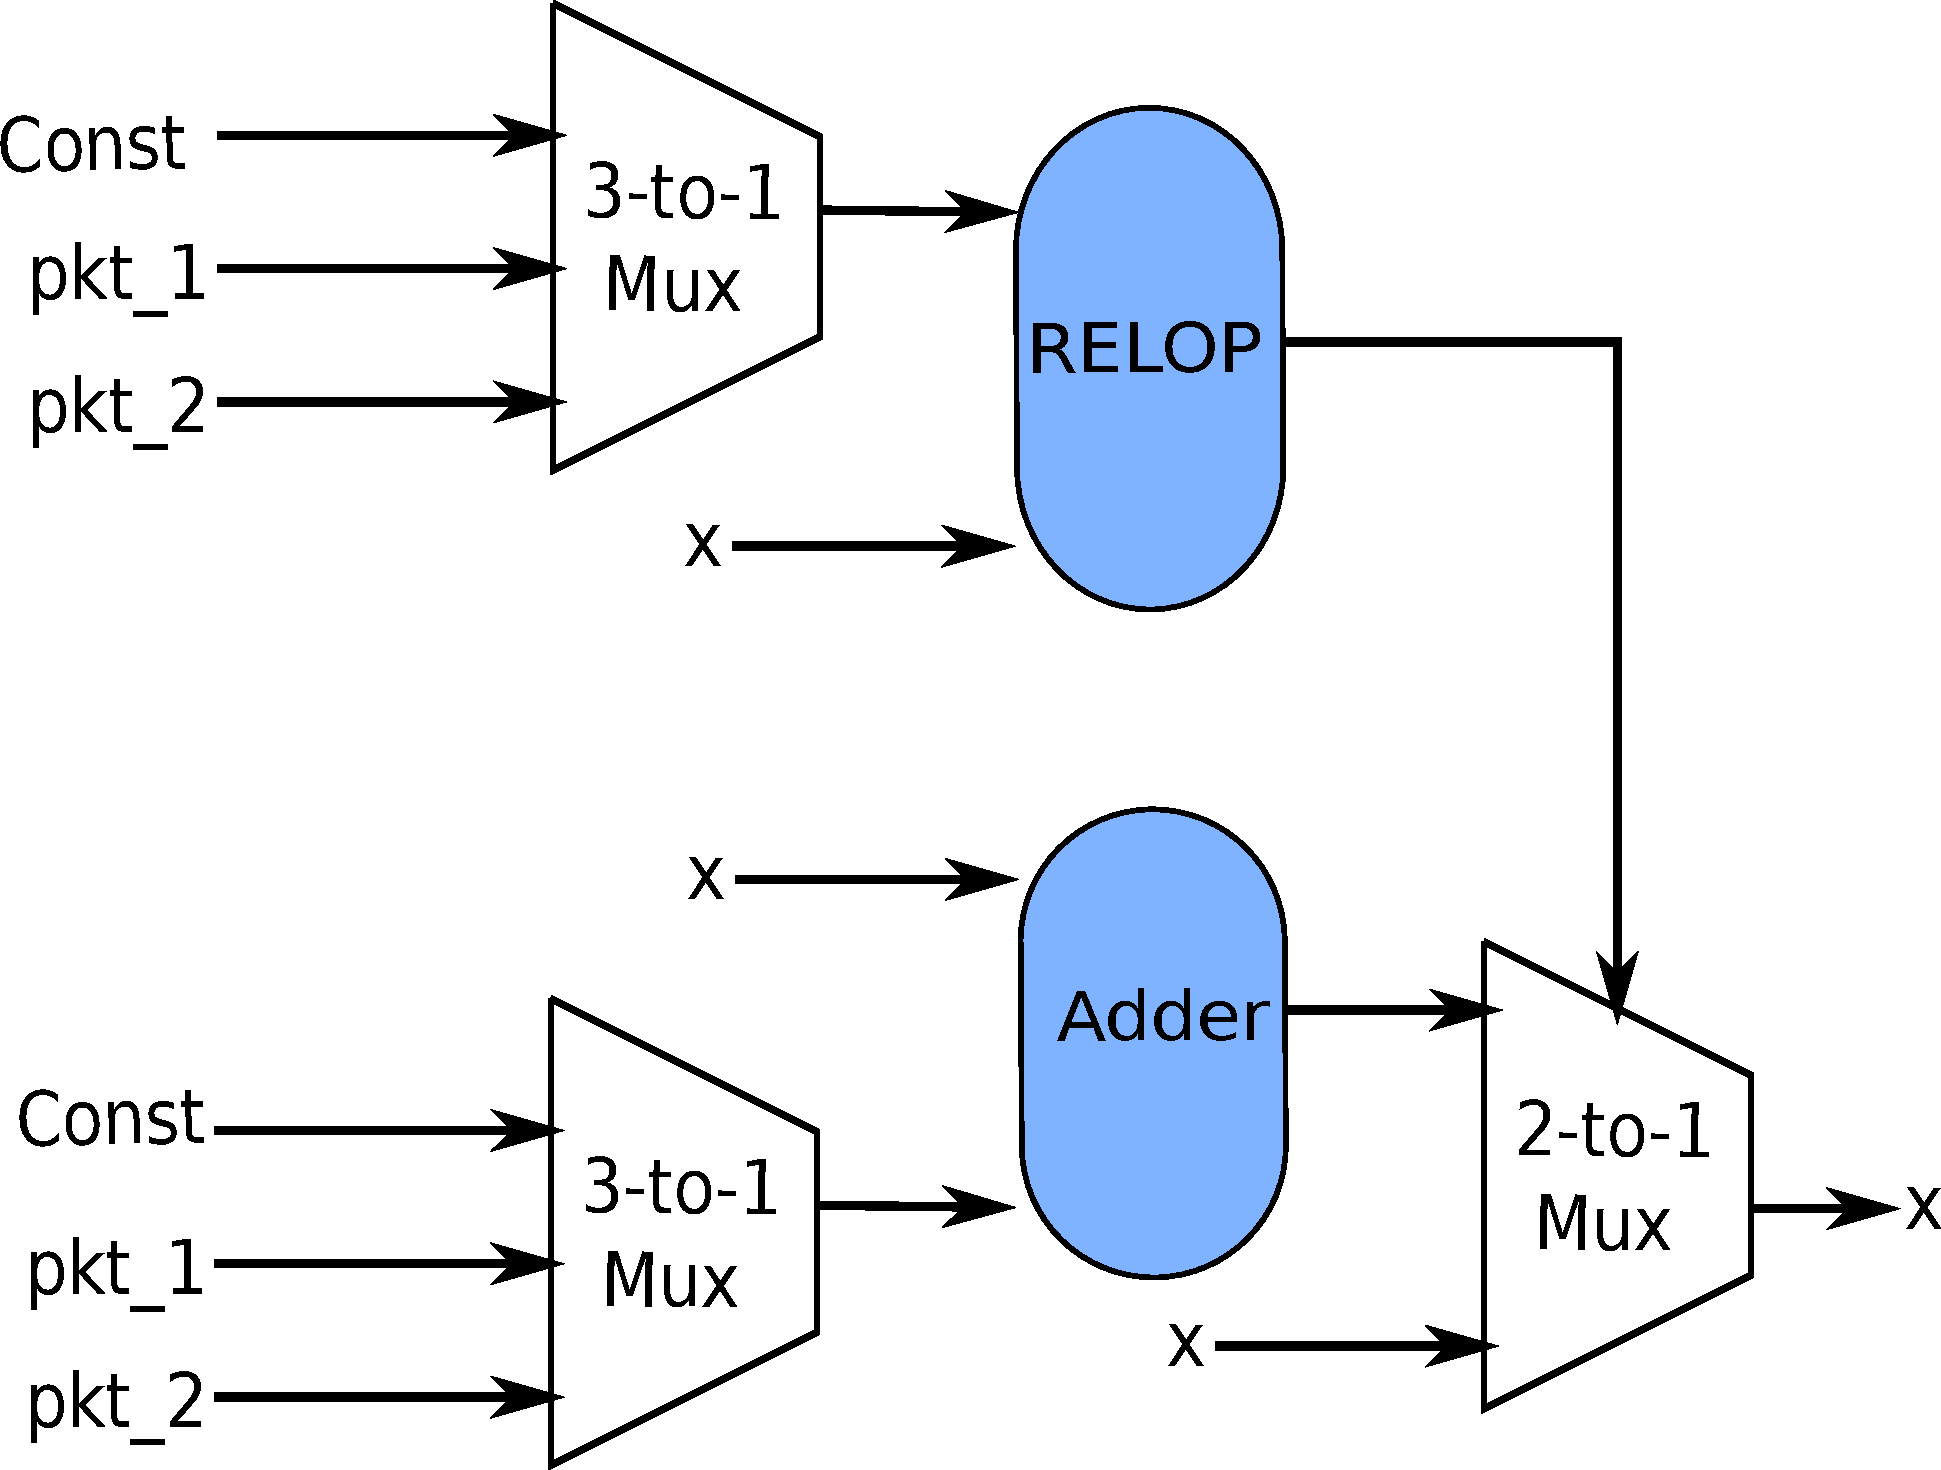
\includegraphics[width=\columnwidth]{pred_raw.pdf}
  \caption{Circuit for PRAW atom with depth 3.}
  \label{fig:praw}
\end{figure*}
\newpage
\begin{figure*}[!htbp]
  \center
  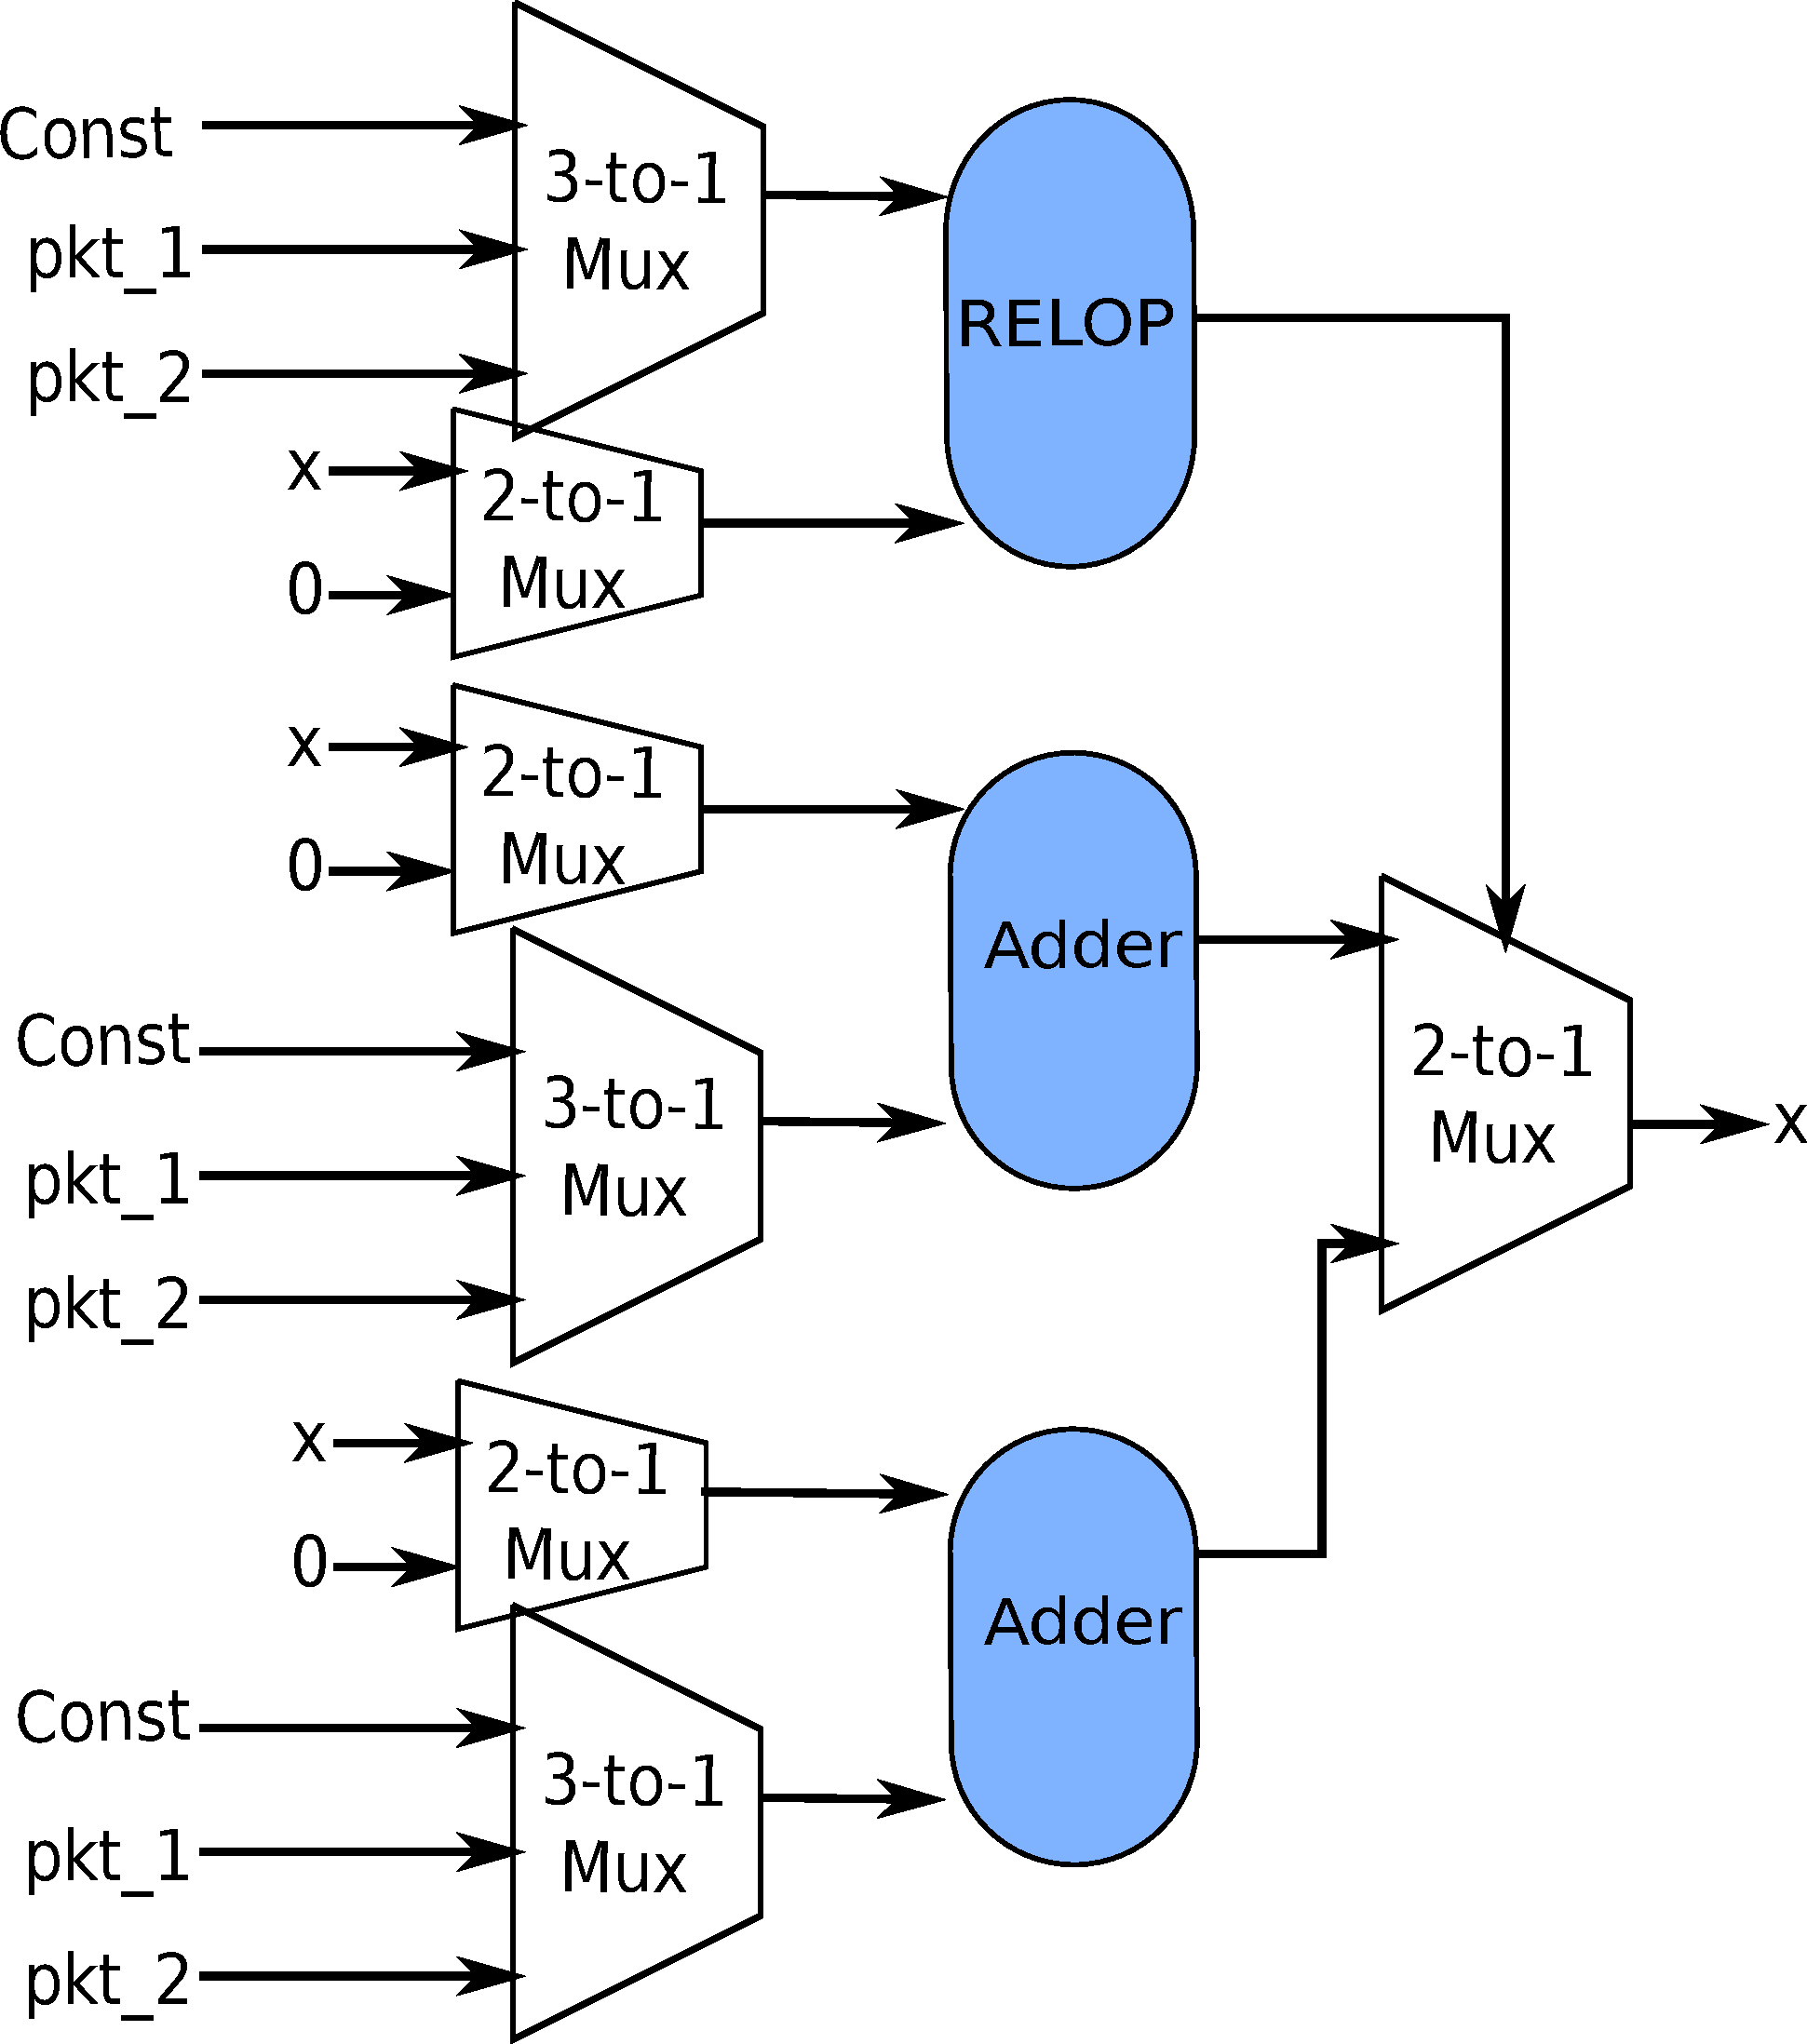
\includegraphics[width=\columnwidth]{if_else.pdf}
  \caption{Circuit for IfElseRAW atom with depth 3.}
  \label{fig:ifelseraw}
\end{figure*}
\begin{figure*}[!htbp]
  \center
  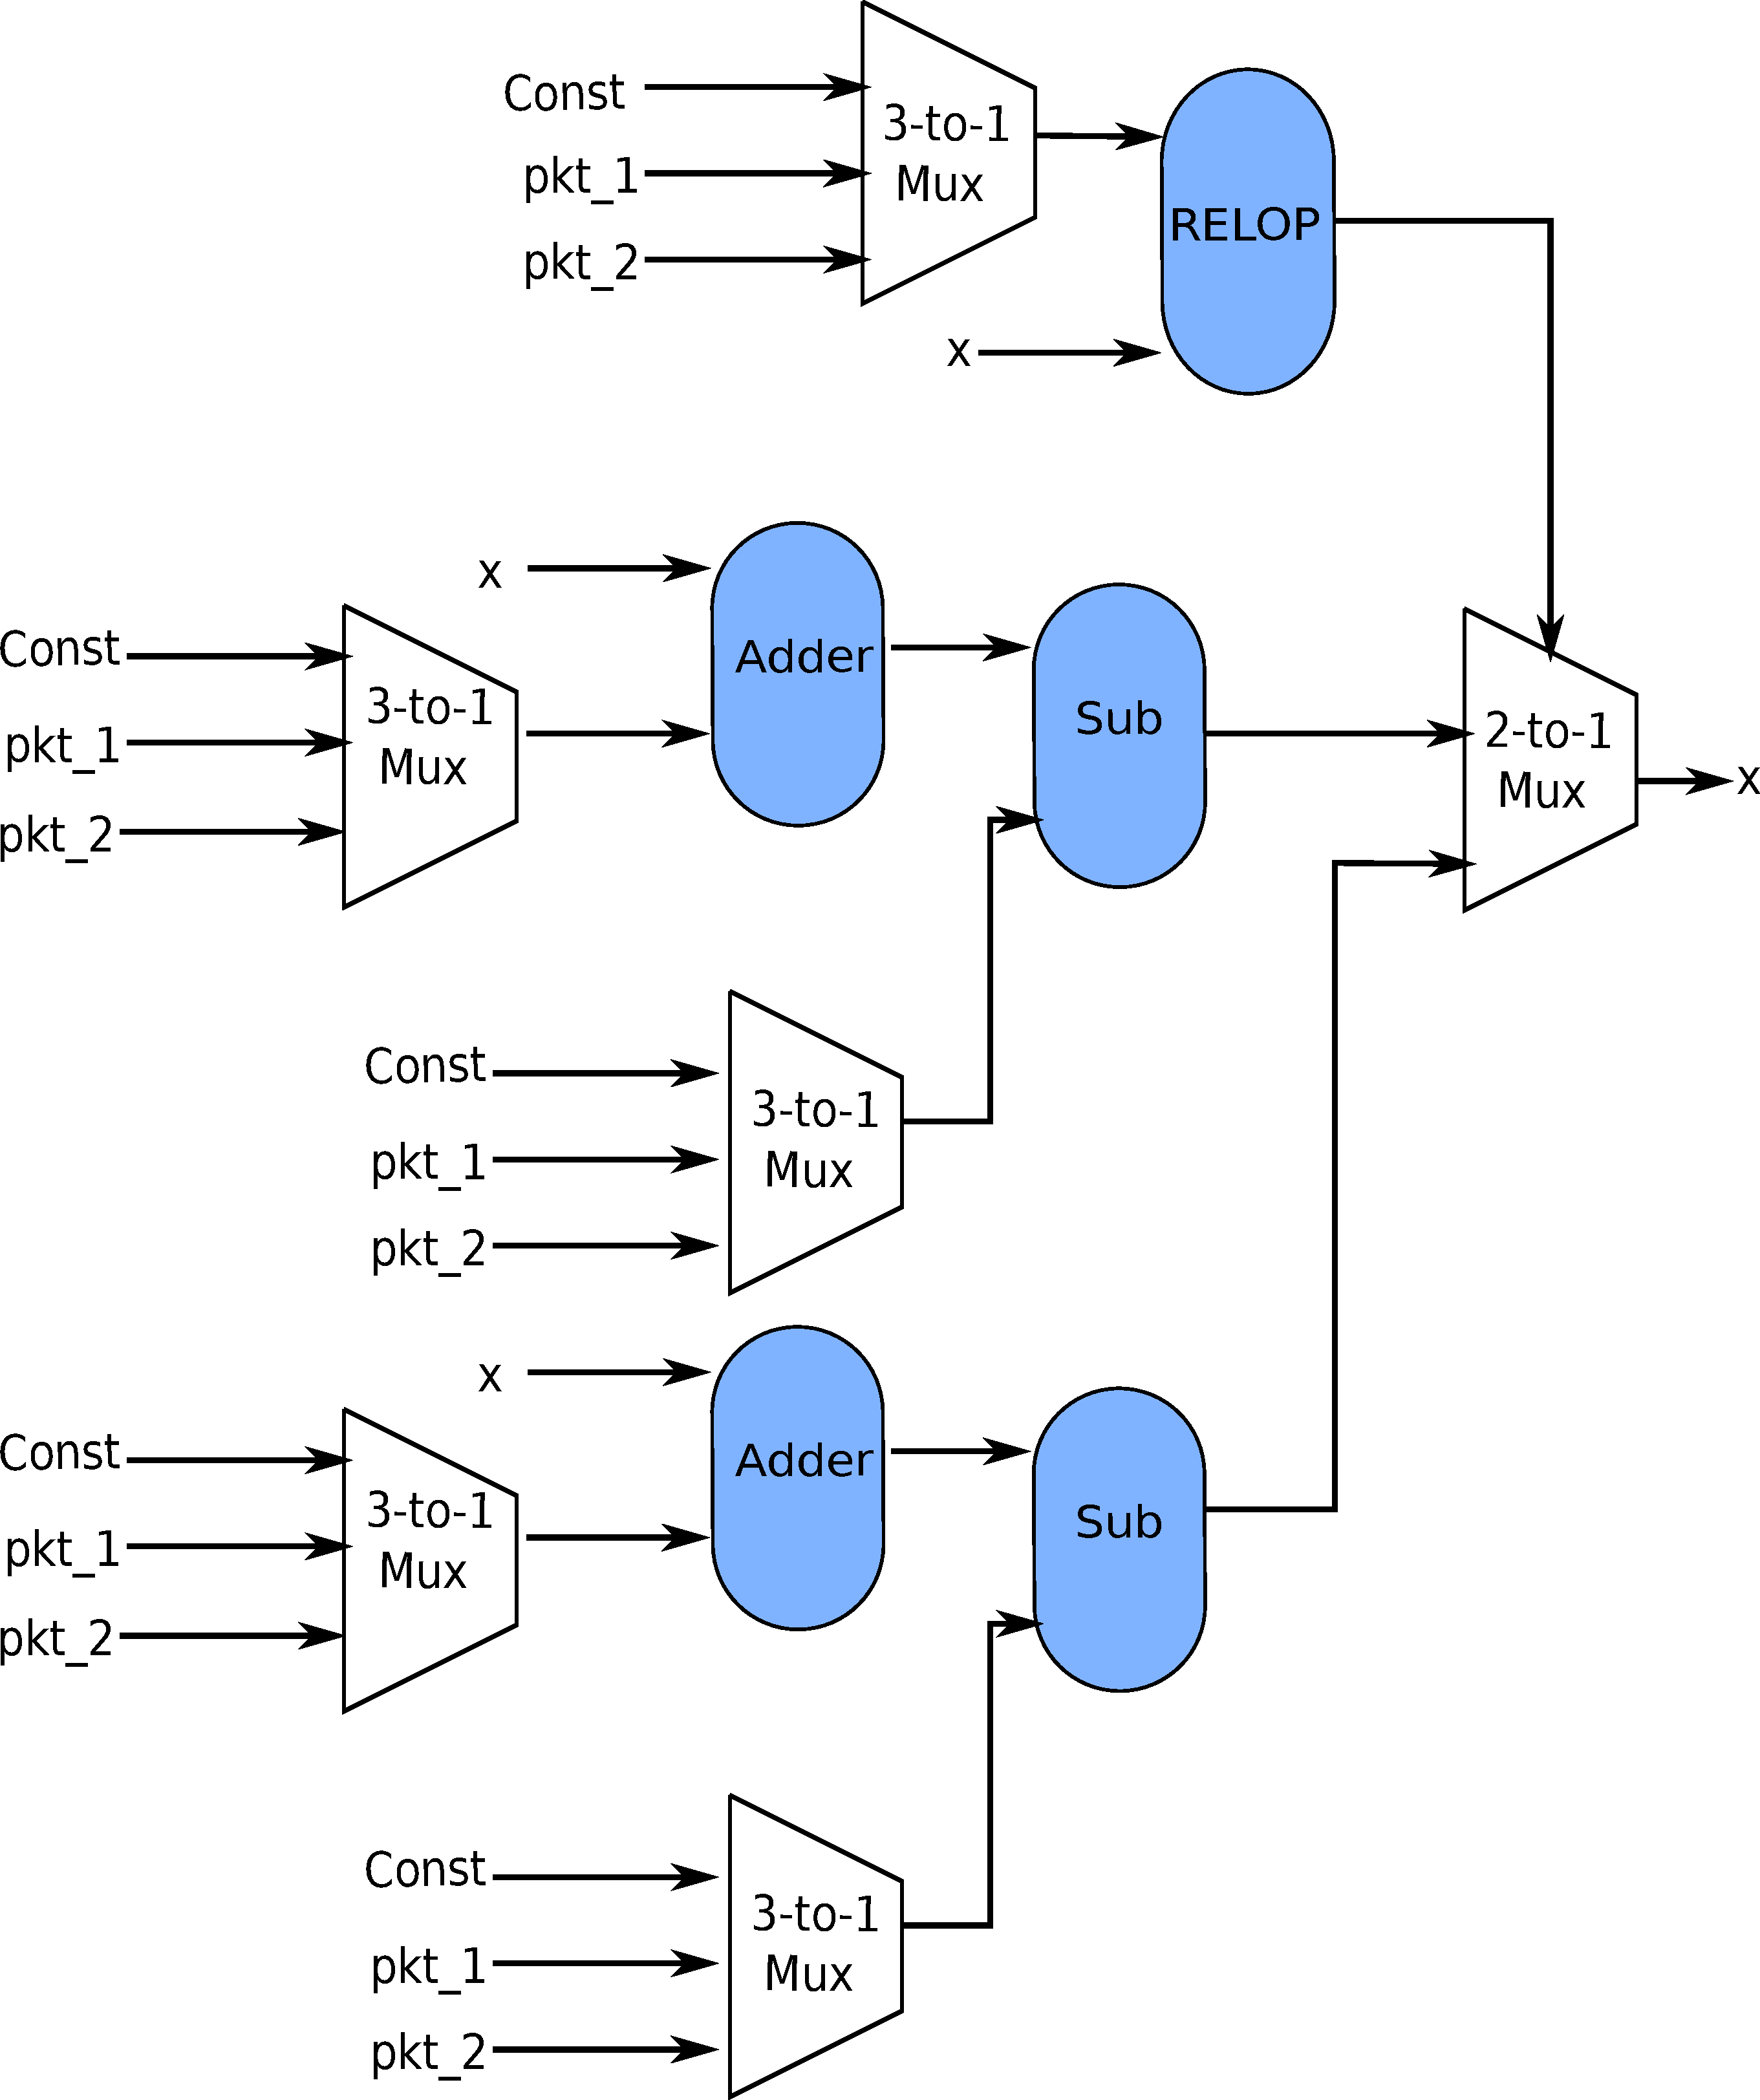
\includegraphics[width=\columnwidth]{sub.pdf}
  \caption{Circuit for Sub atom with depth 4.}
  \label{fig:sub}
\end{figure*}

\newpage
\begin{figure*}[!htbp]
  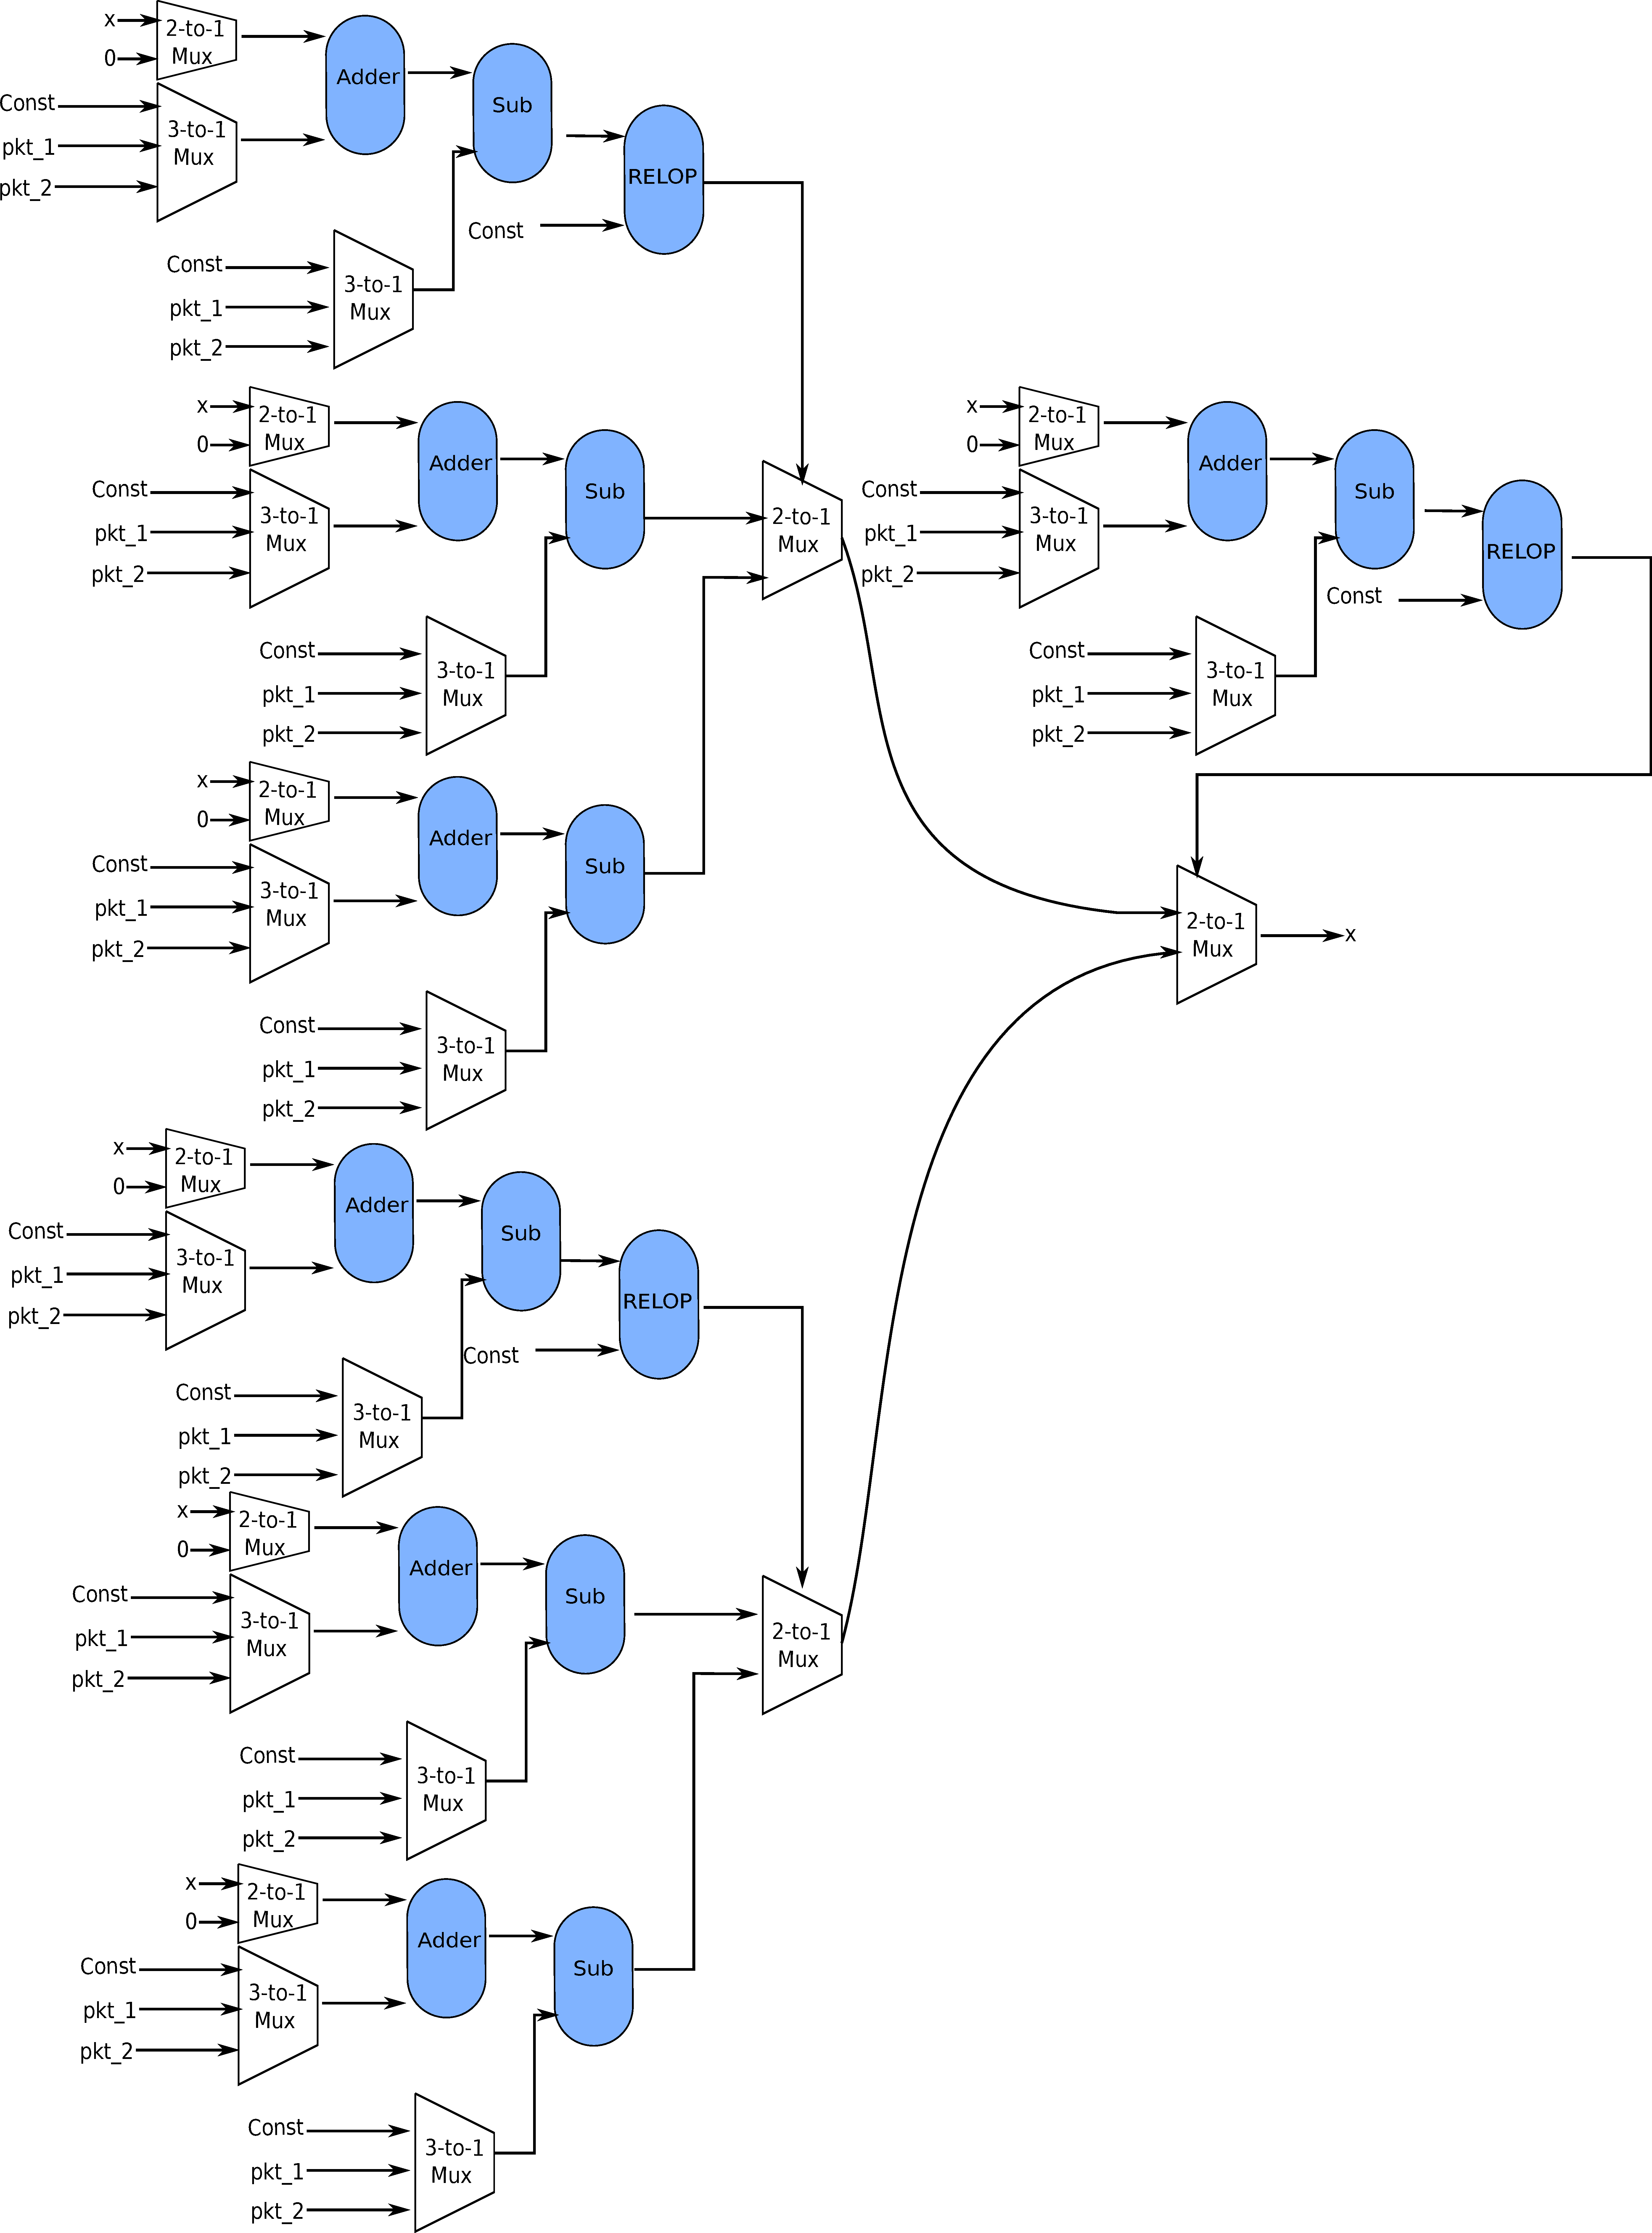
\includegraphics[width=\textwidth]{nested.pdf}
  \caption{Circuit for Nested atom with depth 6.}
  \label{fig:nested}
\end{figure*}

\newpage
\begin{figure*}[!htbp]
  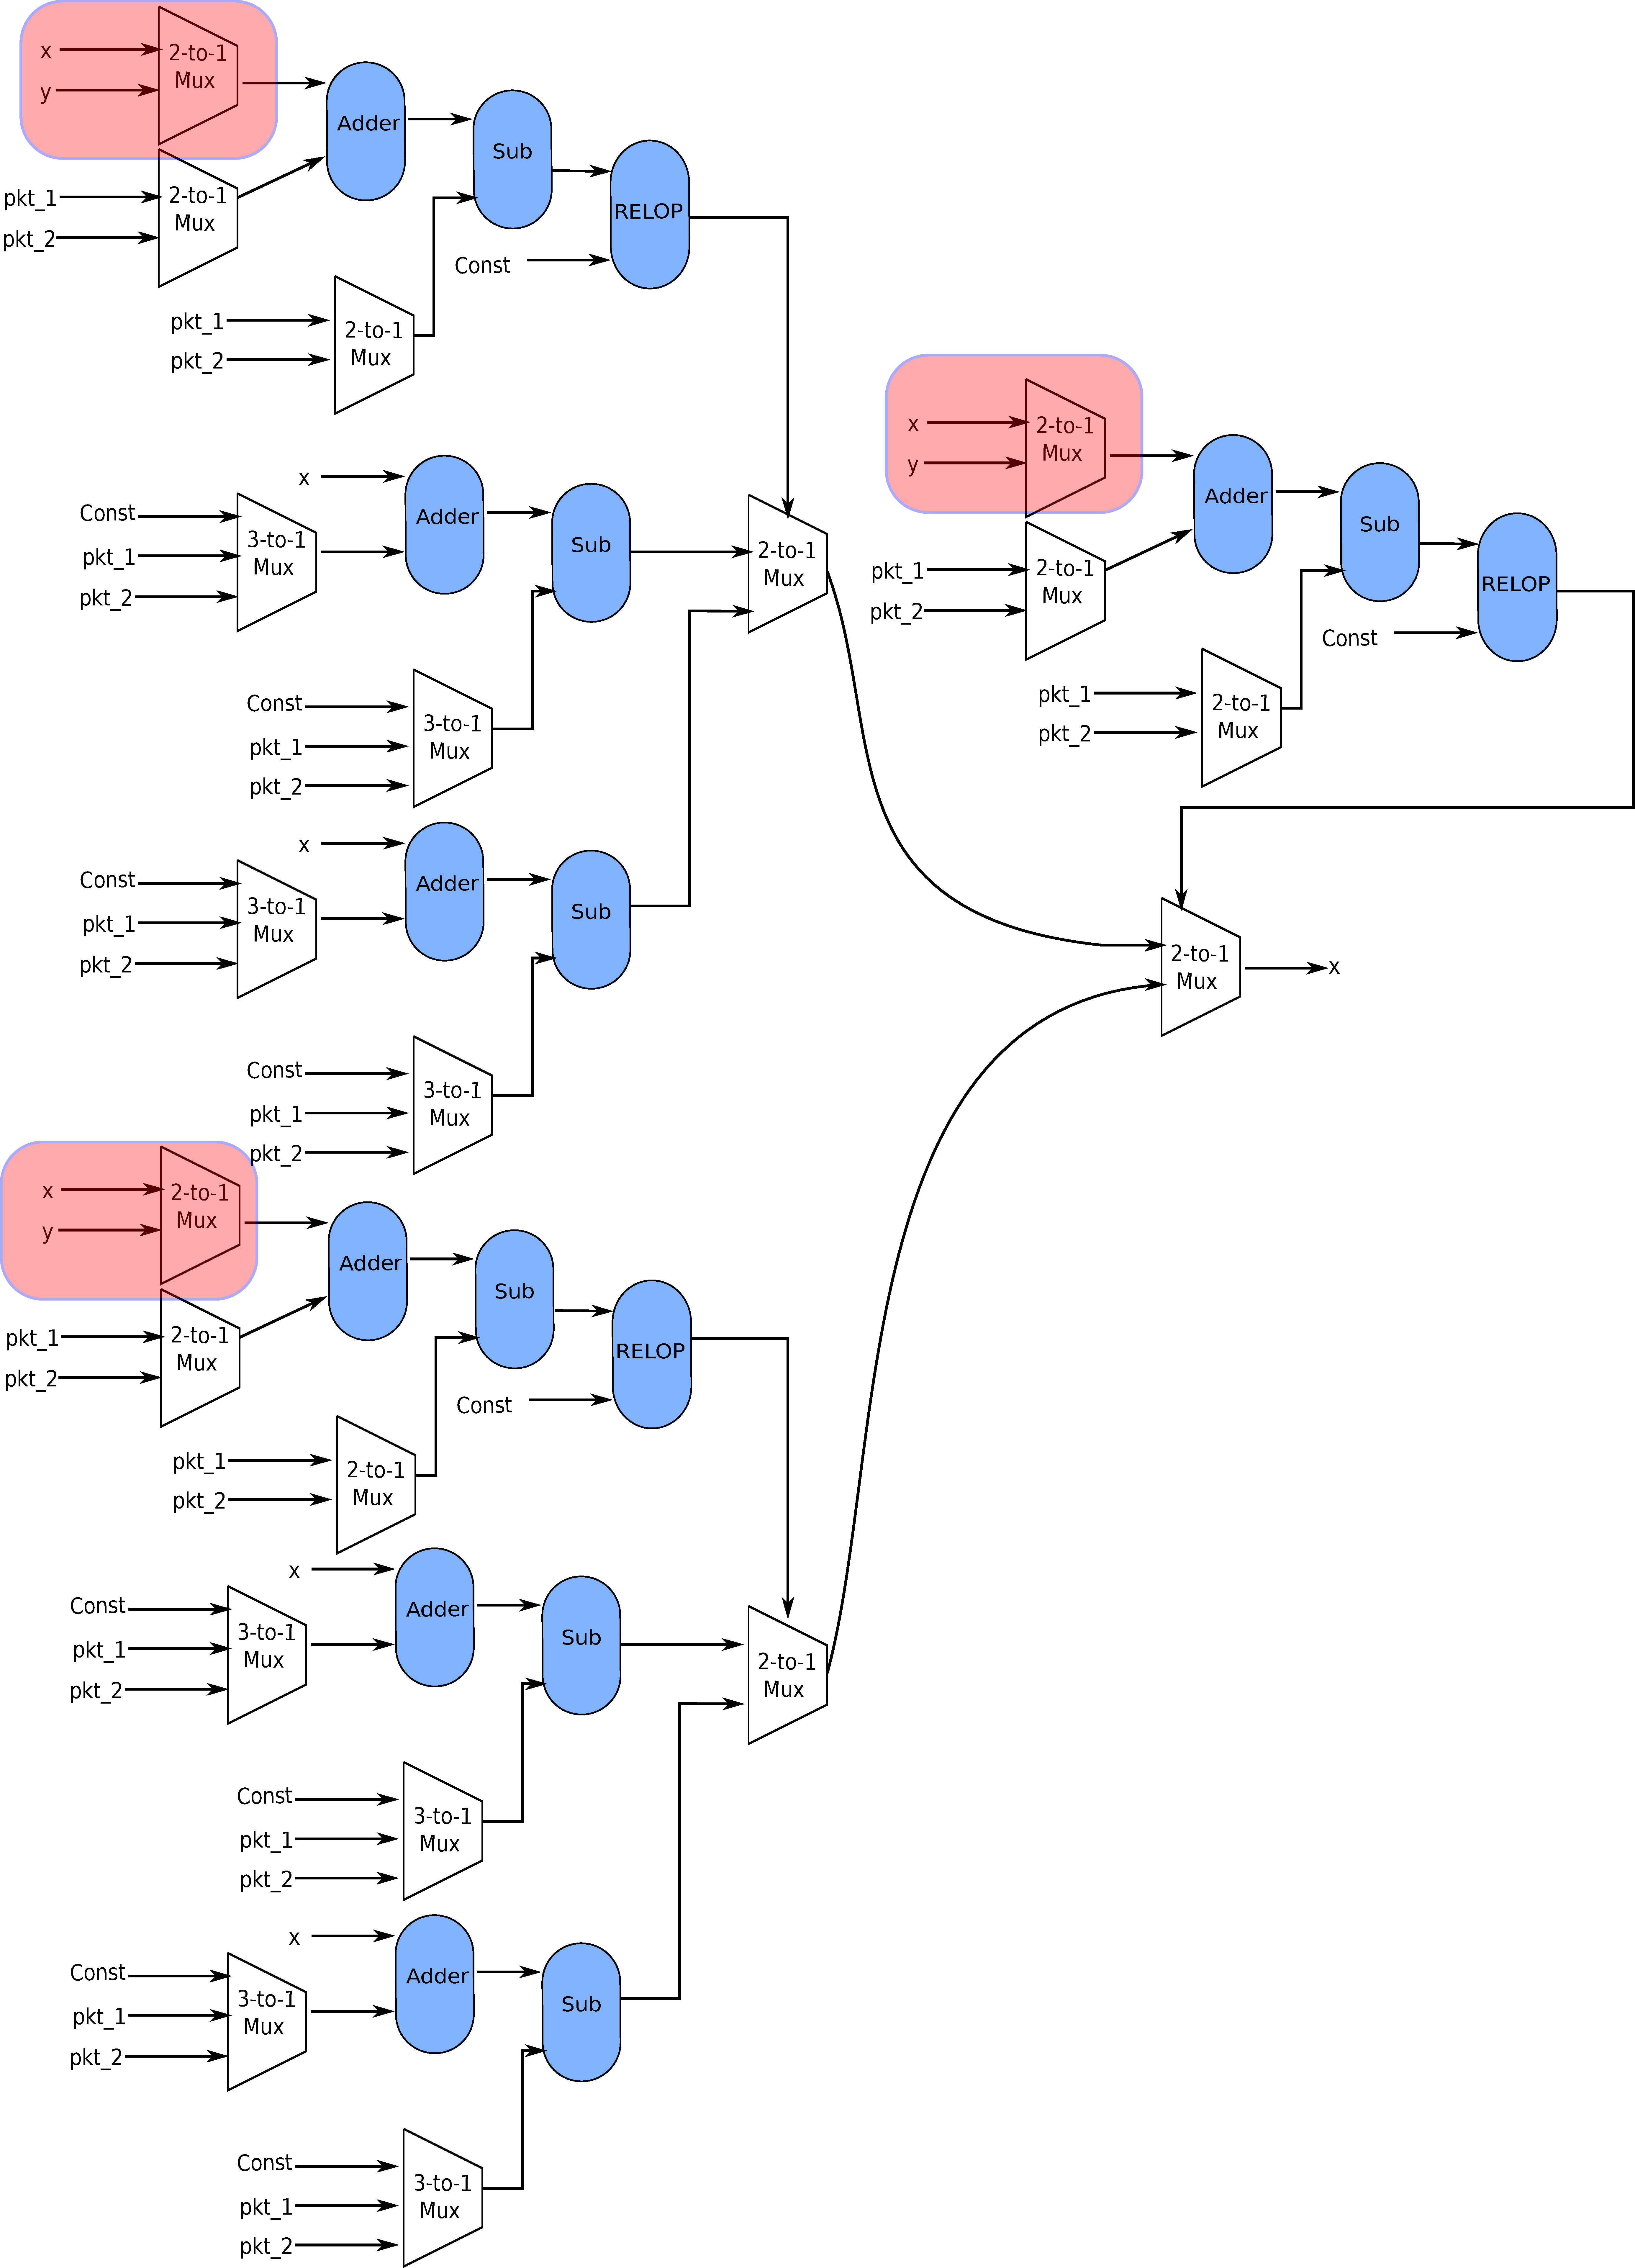
\includegraphics[width=\textwidth]{pairs.pdf}
  \caption{One-half of the circuit for the Pairs atom with depth 6. The other
  half is identical, except that it updates y instead of x, and isn't shown for
simplicity. The shaded regions denote the differences in the Pairs atom
relative to the Nested atom: the predicates can depend on both x and y in the Pairs
atom.}
\label{fig:pairs}
\end{figure*}
